\documentclass[11pt]{article}
\usepackage[a4paper,margin=2.4cm]{geometry}
\usepackage[T1]{fontenc}
\usepackage[utf8]{inputenc}
\usepackage{lmodern}
\usepackage{microtype}
\usepackage{amsmath,amssymb}
\usepackage{booktabs}
\usepackage{graphicx}
\usepackage{xcolor}
\usepackage{tikz}
\usetikzlibrary{positioning,arrows.meta}
\usepackage[numbers,sort&compress]{natbib}
\usepackage[colorlinks=true,linkcolor=blue!50!black,citecolor=blue!50!black,urlcolor=blue!50!black]{hyperref}

\newcommand{\dkv}{\textsc{DecideKV}}
\newcommand{\ms}{\,ms}

\title{\dkv: a Free, Ready-to-Use Tool for Fast Typed Decisions\\with Any Local LLM}
\author{Hobey Garrone\\Independent researcher}
\date{November 2026}

\begin{document}
\maketitle

\begin{abstract}
\dkv{} is a free, open-source Python library (MIT licence, \url{https://github.com/HGarrone/decidekv}) for a common
job: given a state, pick one option from a list, give a level, or answer yes or no, with a local LLM. It is meant to
be versatile and ready to use: one call, any GGUF model that llama.cpp runs (hybrid recurrent models included), lists
from two to tens of thousands of options, and the \texttt{Choice}/\texttt{Score}/\texttt{Noul} question types of
OpenJev. It works without any training, and it can be trained like CLM when examples exist---or without examples, by
letting the LLM label the states. Under equal conditions on one consumer GPU (same model, engine, prompt blocks and
data), \dkv{} is 1.4 to 5.7 times faster than the OpenJev architecture and at least as accurate on six of the seven
task--model pairs we could compare (Banking77 with Qwen3-8B: 63.0\% in 64\ms{} against 39.7\% in 90\ms); it scales to
30{,}000 options where OpenJev stops at 255; with a catalogue trained in minutes it reaches 93.0\% on Banking77 in
16\ms{} and 75.6\% on Typed Decisions without any LLM call, above CLM-8B with heads fine-tuned on the same tasks. The
speed comes from organising the work around the KV cache: option lists stay resident in the cache across states, and
the questions about one state share it through a prefix tree evaluated in one forward pass (a turn of 15 questions on
a 27B hybrid model: from 11.2\,s to 1.4\,s with a long state). We report the weaknesses too: where it is less accurate,
how probabilities depend on batching in llama.cpp, and what we tried that did not work.
\end{abstract}

\section{Introduction}

A large class of LLM uses are not generation but selection: route a customer message to one of 77 intents, map a
definition to one of 30{,}000 words, choose the next tool of an agent, rate a ticket on a 4-level scale, decide
whether a condition holds in a scene. The same option lists are used for thousands of states, and the answer must be
one of the options. Jev-style systems and the open OpenJev library~\citep{openjev} define a clean interface for this
problem with three question types, \texttt{Choice}, \texttt{Score} and \texttt{Noul} (yes/no). Contrastive Language
Models~\citep{clm} answer in about 20\ms{} with heads trained on top of one LLM. Both leave room on the systems side:
OpenJev's design puts the state first and the options after it, so every call recomputes the whole list, and it is
limited to 255 options; CLM's heads belong to one base model and need fine-tuning on the task.

\dkv{} is built as a tool with four goals: (i) \emph{ready to use}: \texttt{pip install}, one call, sensible
defaults; (ii) \emph{fast}: much faster than recomputing the options at every call; (iii) \emph{any model}: any GGUF
model in llama.cpp, including hybrid recurrent ones, and any embedding model; (iv) \emph{no training needed, training
possible}: accurate out of the box, and trainable in minutes when the task has examples. Table~\ref{tab:proscons}
summarises where it stands; the rest of the paper explains how it works and measures every claim.

\begin{table}[t]
\centering\small
\caption{\dkv{} at a glance (numbers from Section~\ref{sec:results}).}\label{tab:proscons}
\begin{tabular}{p{0.47\linewidth}p{0.47\linewidth}}
\toprule
\textbf{Pros} & \textbf{Cons} \\
\midrule
Free (MIT), on GitHub, \texttt{pip install}, one call. &
Less accurate than the OpenJev architecture on Typed Decisions with Qwen3-8B (56.7\% vs 59.3\%). \\ \addlinespace[3pt]
1.4--5.7$\times$ faster than the OpenJev architecture; 15 questions about one state in one forward pass. &
Without training, below CLM-8B fine-tuned on the task where a training set exists. \\ \addlinespace[3pt]
Any GGUF model in llama.cpp, hybrid recurrent models included; any embedding model; three engines. &
Accuracy on open vocabularies falls as the list grows (as for every method). \\ \addlinespace[3pt]
From 2 to 30{,}000+ options (OpenJev: at most 255). &
A head trained on some options hurts the others; the fallback recovers only part of the loss. \\ \addlinespace[3pt]
No training needed; optional training in minutes with numpy, from human labels or from the LLM itself. &
llama.cpp probabilities depend slightly on how the prompt is split into batches. \\ \addlinespace[3pt]
Trained, more accurate than fine-tuned CLM-8B on both tasks with training data, and not tied to one model. &
On hybrid models parallelism is limited to eight sequences; \texttt{full=True} is slow there. \\ \addlinespace[3pt]
Constrained answers (always an option), exclusion of refuted options, probabilities, cascade to the LLM,
semantic cache for repetitive messages. &
Measured on one GPU and one model family (Qwen). \\ \addlinespace[3pt]
\bottomrule
\end{tabular}
\end{table}

\dkv{} takes the opposite design point. The decision is treated as a KV-cache problem: what is shared across calls is
computed once and kept, and only what changes is computed. This paper describes the mechanisms and measures them
under equal conditions. Our contributions are:
\begin{enumerate}
\item \textbf{Resident option prefixes} that persist across states and decisions, implemented with sequence copies in
llama.cpp~\citep{llamacpp}, so that they also work on hybrid recurrent--attention models, where the engine cannot cut
the tail of a sequence and ordinary prefix reuse is unavailable (Section~\ref{sec:resident}).
\item A \textbf{three-level prefix tree} for many questions about one state: state, then one block per option list
shared by several questions, then the questions themselves, decoded in parallel sequences of one forward pass
(Section~\ref{sec:tree}).
\item \textbf{Automatic regimes}: the cached list up to 3{,}000 options, an embedding shortlist above, constrained
decoding through a token trie in both, with exclusion of refuted options (Sections~\ref{sec:decoding},~\ref{sec:catalogue}).
\item A \textbf{trainable catalogue}: a low-rank correction of the embedding space trained with numpy on soft targets,
which can learn from human labels or from the LLM's own probabilities, with a \textbf{fallback} for options without
examples and a \textbf{confidence cascade} to the LLM (Sections~\ref{sec:training}--\ref{sec:cascade}).
\item A measured comparison that reports accuracy and time together, including negative results.
\end{enumerate}
None of the underlying techniques is new on its own (Section~\ref{sec:related}); the contribution is their
combination around the KV cache and the measurements. Two concurrent works, SharedKV-BT~\citep{sharedkvbt} and
LLM-as-Jev~\citep{llmasjev}, score the candidates of several typed fields over a context encoded once; we discuss the
differences in Section~\ref{sec:related}.

\section{Method}

\begin{figure}[t]
\centering
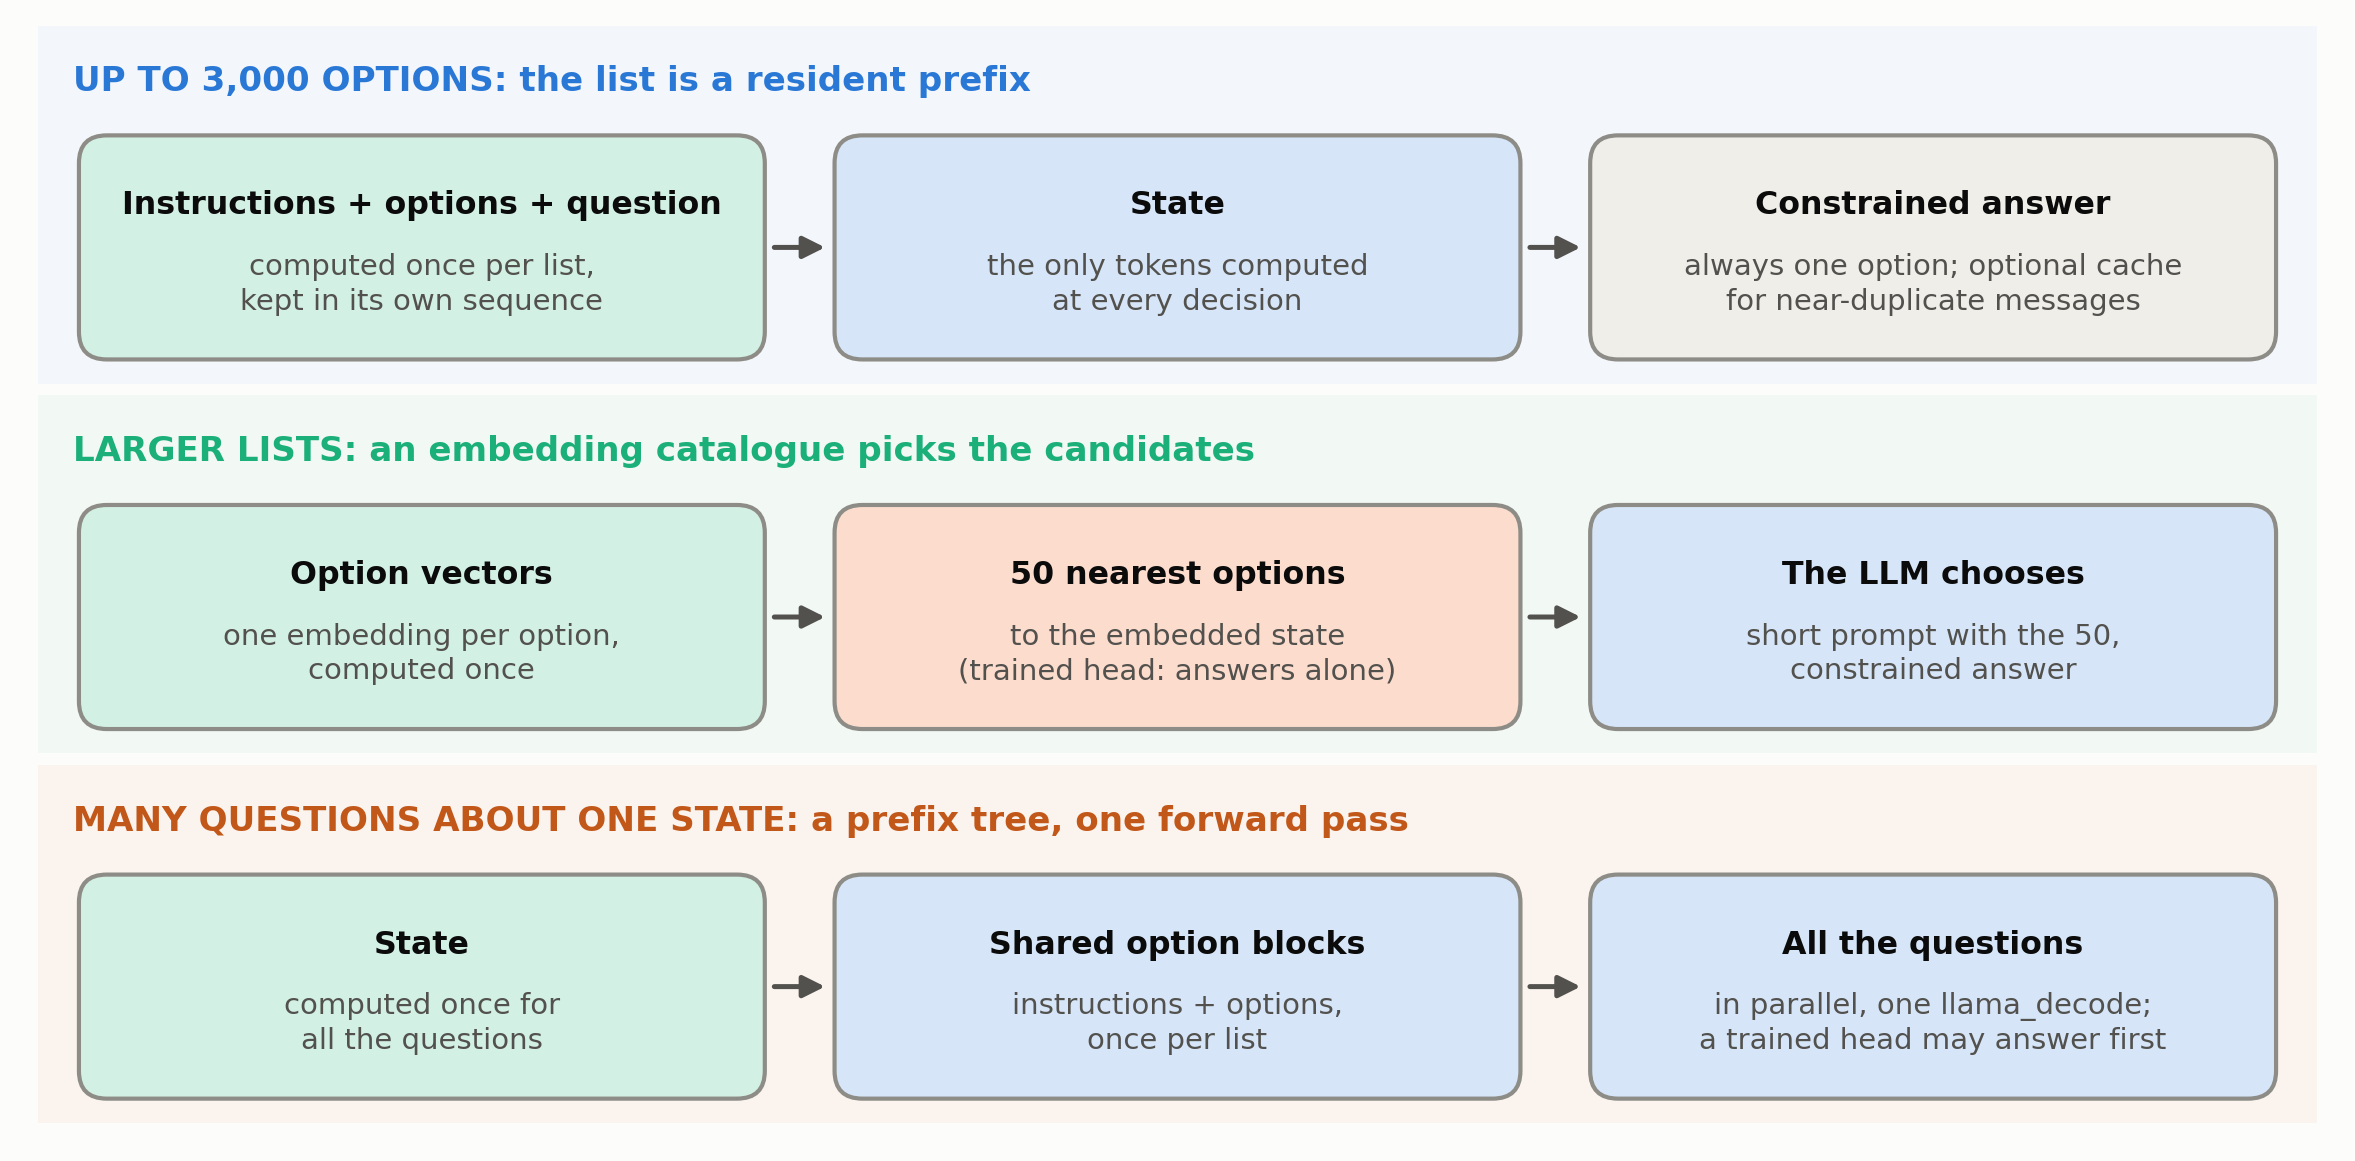
\includegraphics[width=\linewidth]{fig_overview.png}
\caption{Overview of \dkv. Top: up to 3{,}000 options the instructions and the options are a resident prefix, computed
once, and every decision computes only the state and the question. Middle: for larger lists an embedding catalogue
picks 50 candidates for the LLM (with a trained head, the catalogue answers alone). Bottom: many questions about one
state are answered as a prefix tree in one forward pass; a trained head can answer first and pass only uncertain or
unfamiliar questions to the LLM.}\label{fig:overview}
\end{figure}

\subsection{Background: the KV cache}
An LLM reads its prompt as a sequence of tokens. For every token and every layer it computes a key vector and a value
vector; later tokens attend to the keys and values of all earlier tokens. These vectors form the \emph{KV cache}.
Reading the prompt (the \emph{prefill}) is the expensive part of a short decision: producing a one-token answer
afterwards costs little. In a causal model the keys and values of a token depend only on the tokens before it, so two
prompts that start with the same text have the same cache for that text, and it can be computed once and reused.
Serving systems use this to share common prefixes between requests~\citep{vllm,sglang}; \dkv{} builds the whole
decision around it: what is constant goes first and is kept, what changes goes after it.

\subsection{Typed decisions}
\paragraph{A worked example.} A support application receives the message \emph{``This is the third time I write! My
card was stolen yesterday and nobody answers.''} and asks three questions about it: which request it is (a
\texttt{Choice} among \emph{lost or stolen card}, \emph{refund}, \emph{card arrival}), how upset the customer is (a
\texttt{Score} with levels \emph{calm}, \emph{annoyed}, \emph{furious}), and whether to escalate it to a human now (a
\texttt{Noul}). Every decision is built from four pieces, which we name as in OpenJev~\citep{openjev}:
\begin{center}\small
\begin{tabular}{lll}
\toprule
Piece & In the example & Changes \\
\midrule
\emph{state} & the customer's message & at every message \\
\emph{instructions} & a fixed sentence telling the model how to answer & never (depends on the question type) \\
\emph{options} & the three requests; the three levels; \texttt{Yes}/\texttt{No} & never \\
\emph{question} & ``How upset is the customer?'' & never, but differs between questions \\
\bottomrule
\end{tabular}
\end{center}
In a real application almost all the text is fixed and only the state changes, so \dkv{} puts everything fixed
first. For a list asked its own question (one list, many states) the prompt of the \texttt{Score} question is (exact
text, inside the model's chat template):
\begin{center}
\begin{minipage}{0.92\linewidth}\footnotesize
\begin{verbatim}
You are a decision engine. Answer the question about the state by choosing one
level from the list of levels. Reply with the label of the level (the text before
the colon), and nothing else.                                    <- instructions
### Levels
0: calm
1: annoyed
2: furious                                                       <- options
### Question
How upset is the customer? Answer with the level number.         <- question
### State
customer: This is the third time I write! My card was stolen ... <- state
### Level                                                        <- answer head
\end{verbatim}
\end{minipage}
\end{center}
Everything above the state is one cached prefix; at every decision only the state and the answer head are computed.
The model's next token is the answer, and the probabilities of the tokens \texttt{0}, \texttt{1}, \texttt{2} give the
probability of every level. Putting the question before the state was never less accurate than putting it after
(Section~\ref{sec:results}) and saves its tokens at every decision. When several questions share one list, as in
the example's \texttt{Noul} questions, the list stays one cached prefix and each question goes after the state, so
that the questions do not compete for the cache (Section~\ref{sec:tree}).

\paragraph{Question types.} A decision is a state $s$ (any text or structured object) and a question $q$ with an option list $O_q$. A
\texttt{Choice} picks one option; a \texttt{Score} picks one of $n$ levels described by criteria; a \texttt{Noul}
answers yes or no. \texttt{Score} and \texttt{Noul} use single-token labels (\texttt{0}..\texttt{n-1}, \texttt{Yes}/\texttt{No})
and return the probability of every level; a \texttt{Choice} is answered by decoding the option's name. Every prompt
is made of the same blocks for every method we measure: instructions, the option block, the state, the question and
an answer head, written in the model's chat template with thinking disabled.

\subsection{Resident option prefixes}\label{sec:resident}
In a causal LLM the keys and values of a token depend only on the tokens before it. If the prompt starts with the
instructions and the option block $P_q$, the KV cache of $P_q$ is the same for every state and can be computed once.
\dkv{} keeps each such prefix in a llama.cpp sequence of its own (a \emph{resident prefix}). At every decision the
resident sequence is copied into the working sequence and only the state, the question and the answer head are
evaluated. On attention layers the copy shares cache cells and costs nothing; on recurrent layers the recurrent state
is copied, a few milliseconds. This is what makes reuse possible on hybrid models such as Qwen3.5/3.8: the engine
cannot remove the tail of a recurrent sequence, so the usual ``longest common prefix'' reuse does not apply. Several
lists stay resident at once with least-recently-used eviction; we keep seven by default because, in our measurements,
llama.cpp decodes hybrid models up to ten times slower beyond eight sequences in total.

\subsection{Constrained decoding and probabilities}\label{sec:decoding}
A \texttt{Choice} is decoded greedily through a token trie of the option names~\citep{genre}, so the answer is always
an option; options already refuted (for instance cells already shot in a game) are removed from the trie. With
\texttt{full=True} the log-probability of every option is computed by evaluating all trie paths in parallel
sequences of one batch, with a probability floor of $10^{-6}$ to prune branches; on Qwen3-8B this costs 50\ms{} for
77 options against 66\ms{} for greedy decoding, exact to $6\times 10^{-6}$ with respect to scoring each option alone.

\subsection{Many questions about one state: the prefix tree}\label{sec:tree}
A typical agent step asks many questions about one state (our motivating application asks 15 per message: 4
\texttt{Score} and 11 \texttt{Noul}). With the options first, the state is recomputed for every question. \dkv{}
instead orders the prompt as [state] [instructions + options] [question + answer head] and builds a tree
(Figure~\ref{fig:tree}): the state is evaluated once as a resident prefix; every option block used by at least two
questions is evaluated once on a copy of the state; then every question---or, for an option block used once, the block
and its question---is evaluated in its own sequence copied from its parent, all in one \texttt{llama\_decode}, keeping
the logits of the last token of each sequence. On hybrid models the number of parallel sequences is bounded by the
eight-sequence limit, so the questions run in groups, and the least recently used resident lists are freed when
the tree needs the sequences. The order is chosen automatically: questions with a short option
block (at most 2{,}000 characters, or shorter than the state) share the state when there are at least two of them;
long lists stay options-first and resident across states.

\begin{figure}[t]
\centering
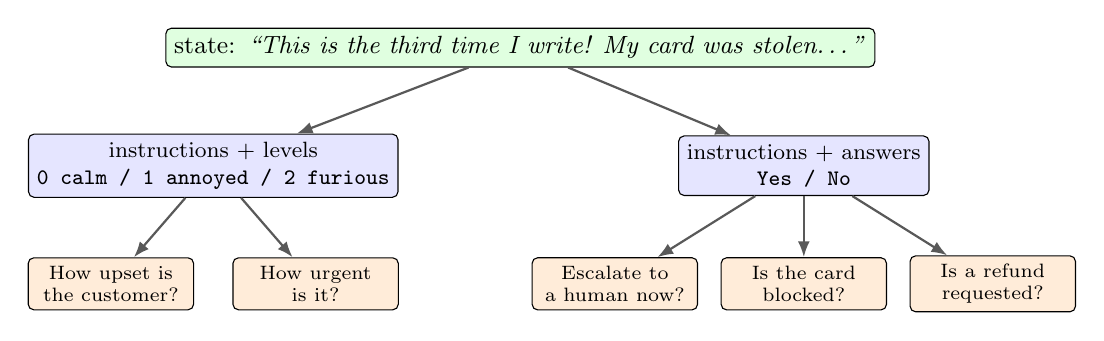
\begin{tikzpicture}[
  box/.style={draw, rounded corners=2pt, align=center, inner sep=3pt},
  st/.style={box, fill=green!12, font=\small},
  bl/.style={box, fill=blue!10, font=\footnotesize},
  q/.style={box, fill=orange!15, font=\scriptsize, minimum width=2.1cm},
  arr/.style={-{Latex[length=2mm]}, thick, gray!70!black}]
\node[st] (s) at (0, 0) {state: \emph{``This is the third time I write! My card was stolen\dots''}};
\node[bl] (b1) at (-3.9, -1.5) {instructions + levels\\\texttt{0 calm / 1 annoyed / 2 furious}};
\node[bl] (b2) at (3.6, -1.5) {instructions + answers\\\texttt{Yes / No}};
\node[q] (q1) at (-5.2, -3.0) {How upset is\\the customer?};
\node[q] (q2) at (-2.6, -3.0) {How urgent\\is it?};
\node[q] (q3) at (1.2, -3.0) {Escalate to\\a human now?};
\node[q] (q4) at (3.6, -3.0) {Is the card\\blocked?};
\node[q] (q5) at (6.0, -3.0) {Is a refund\\requested?};
\draw[arr] (s) -- (b1); \draw[arr] (s) -- (b2);
\foreach \x in {q1,q2} \draw[arr] (b1) -- (\x);
\foreach \x in {q3,q4,q5} \draw[arr] (b2) -- (\x);
\end{tikzpicture}
\caption{Prefix tree for five questions about one message (two \texttt{Score}, three \texttt{Noul}). Green: the
state, computed once. Blue: the instructions and options of a list, computed once on a copy of the state and shared by
the questions that use that list. Orange: the questions, each in its own sequence copied from its block, all evaluated
in one \texttt{llama\_decode}; the last token of each sequence gives that question's answer. Without the tree the
state would be read five times and each option block several times.}\label{fig:tree}
\end{figure}

\subsection{Large lists: the embedding catalogue}\label{sec:catalogue}
The cache of a list grows with the list (about 78\,KB per token for Qwen3-8B with an 8-bit cache), and beyond a few
thousand options it no longer fits the context. Above a threshold (3{,}000 options by default) \dkv{} keeps one
embedding per option, shortlists the 50 options closest to the state, writes only these in the prompt and decodes
through their trie. This is the standard retrieve-then-rerank pipeline; any embedding model can be used.

\subsection{Trainable catalogue}\label{sec:training}
With examples, the catalogue can be trained. States and options are embedded by a frozen encoder ($x_s$, $x_o$) and
corrected by low-rank maps that start from the identity:
\begin{equation}
z_s = \frac{x_s + (x_s U_s) V_s^\top}{\lVert \cdot \rVert},\qquad
z_o = \frac{x_o + (x_o U_o) V_o^\top}{\lVert \cdot \rVert},\qquad
p(o\mid s) = \operatorname{softmax}_{o\in C(s)}\!\big(\tau\, z_s^\top z_o\big),
\end{equation}
Here $x_s, x_o \in \mathbb{R}^{d}$ are the embedding vectors of the state text and of an option text ($d=2{,}560$ for
Qwen3-Embedding-4B). $U_s, V_s$ (for states) and $U_o, V_o$ (for options) are the trained parameters: matrices of
size $d \times r$ with rank $r=64$, so that $(x U)V^\top$ is a low-rank correction added to the original vector
(about 650{,}000 parameters in total). $V_s$ and $V_o$ start at zero, so before training $z_s$ and $z_o$ are the
original embeddings and the trained catalogue starts exactly from the untrained one. The denominator
$\lVert\cdot\rVert$ is the Euclidean norm of the numerator: it rescales the corrected vector to length one, so that
$z_s^\top z_o$ is the cosine similarity between the corrected state and option. $\tau=30$ is a fixed temperature
that turns cosines (between $-1$ and $1$) into well-separated logits, and $C(s)$ is the set of candidate options
of the example. For typed questions every example has its own candidate set (the options of its question) and a
\emph{soft} target distribution $t$: a one-hot vector for a hard label, the
official distribution of a dataset, or the probabilities that an LLM assigns to every option. The loss is the
cross-entropy $-\sum_o t_o \log p(o\mid s)$ (an InfoNCE-style objective~\citep{infonce,clip} over per-example
candidates), optimised with Adam in numpy; the weights of the best validation epoch are kept. The LLM is never
trained. The function \texttt{teach} lets the LLM label a set of states with full distributions, so the catalogue can
be trained without any human label; it then learns to reproduce its teacher at the cost of the embedding calls.

\subsection{Fallback for options without examples}\label{sec:fallback}
A head trained on some options gets the others wrong, and confidently: on Banking77 its margin does not separate
these errors. The head therefore records which options had examples. When the \emph{untrained} catalogue prefers an
option without examples and disagrees with the trained one, the LLM chooses among the five best options of each
catalogue. A head trained on every option never falls back.

\subsection{Confidence cascade}\label{sec:cascade}
With a trained head and a threshold $T \in [0, 1]$, the catalogue answers every question, and the questions whose
answer has a confidence below $T$ are asked to the LLM in one call (through the prefix tree). The confidence of an
answer with probabilities $p = (p_1, \dots, p_{|C|})$ over its $|C|$ options is
\begin{equation}
\mathrm{conf}(p) = 1 - \frac{H(p)}{\log |C|}, \qquad H(p) = -\sum_{i=1}^{|C|} p_i \log p_i ,
\end{equation}
where $H(p)$ is the entropy of the answer distribution and $\log|C|$ its maximum value (all options equally likely):
the confidence is 1 when all the probability is on one option and 0 when it is spread evenly (the definition used by
OpenJev). For example, $p=(0.02, 0.15, 0.83)$ over three levels gives a confidence of 0.53.

\subsection{Engines}
The default engine runs llama.cpp in the Python process on the GGUF files downloaded by Ollama. A
\texttt{llama-server} engine gives each resident prefix a server slot and decodes with a grammar of the option names;
an Ollama engine is also provided, without resident prefixes on hybrid models.

\section{Experimental setup}
All measurements use one NVIDIA RTX 4070 SUPER (12\,GB). Models: Qwen3-8B~\citep{qwen3} (36 attention layers,
Q4\_K\_M) and Qwen3.8-27B in IQ2\_S quantisation (architecture \texttt{qwen35}, recurrent and attention layers), with an
8-bit KV cache; embeddings from Qwen3-Embedding-4B. Tasks: Banking77~\citep{banking77} (77 intents, 300 test
messages, 10{,}003 training messages); a WordNet~\citep{wordnet} reverse dictionary (definition to word) with 200 to
30{,}000 candidate nouns; Typed Decisions~\citep{typeddecisions} (400 test cases with five typed questions each, 2{,}000
decisions; 1{,}200 training cases; 20 distinct questions); and an aim game on a $15\times15$ grid (20 games, at most 25
shots, refuted cells excluded). Every method measured by our scripts uses the same model, engine, prompt blocks and
queries; the differences come only from the architecture. ``OpenJev architecture'' is OpenJev's design (state first,
options after it, answer read from the logit of the first token of each option) re-implemented on the shared prompt and
engine; it is not the OpenJev library. The rows ``OpenJev library'' (its own prompt, through Ollama) and ``CLM-8B''
(Qwen3-8B with the released CLM-v0.1-8B heads, as released or with heads fine-tuned on the task) come from earlier
measurements on the same machine and weights. Every cell reports accuracy and the median time of one decision.
With 300 queries one accuracy has a standard error of about 3 points; times vary by a few percent between sessions.

\section{Results}\label{sec:results}

\subsection{Comparison under equal conditions}
Table~\ref{tab:comparison} compares the methods on Qwen3-8B. Without training, \dkv{} is ahead of the OpenJev
architecture on Banking77, WordNet and the aim game, and behind it on Typed Decisions; it is 1.4--3.7 times faster.
CLM-8B as released is far behind on every task; with heads fine-tuned on the task it is ahead of untrained \dkv{} where
a training set exists. With a trained catalogue \dkv{} is ahead of fine-tuned CLM-8B on both tasks with training data.

\begin{table}[t]
\centering\small
\caption{Accuracy $\cdot$ median time per decision on Qwen3-8B. Bold: the best accuracy and the lowest time of
each column. ``--'': not applicable or not measured.}\label{tab:comparison}
\resizebox{\linewidth}{!}{\begin{tabular}{lllll}
\toprule
Method & Banking77 & WordNet-200 & Typed Decisions & Aim game (won) \\
\midrule
\dkv & 63.0\% $\cdot$ 64\ms & \textbf{74.7\%} $\cdot$ 36\ms & 56.7\% $\cdot$ \textbf{41\ms} & \textbf{100\%} $\cdot$ 160\ms \\
\dkv, trained catalogue & \textbf{93.0\%} $\cdot$ \textbf{15\ms} & -- & \textbf{75.6\%} $\cdot$ 57\ms & -- \\
OpenJev architecture & 39.7\% $\cdot$ 90\ms & 63.3\% $\cdot$ 132\ms & 59.3\% $\cdot$ 67\ms & 25.0\% $\cdot$ 423\ms \\
OpenJev library (Ollama) & 44.0\% $\cdot$ 117\ms & 22.7\% $\cdot$ 164\ms & 58.1\% $\cdot$ 62\ms & 25.0\% $\cdot$ 469\ms \\
CLM-8B as released & 4.3\% $\cdot$ 35\ms & 12.7\% $\cdot$ \textbf{21\ms} & 36.8\% $\cdot$ 79\ms & 15.0\% $\cdot$ \textbf{124\ms} \\
CLM-8B, heads fine-tuned & 84.3\% $\cdot$ 21\ms & 26.0\% $\cdot$ \textbf{21\ms} & 71.0\% $\cdot$ 79\ms & -- \\
Embedding model alone & 65.7\% $\cdot$ 16\ms & -- & -- & -- \\
Embedding top-50, then LLM & 58.3\% $\cdot$ 127\ms & -- & -- & -- \\
Cross-encoder (30 messages) & 70.0\% $\cdot$ 1{,}589\ms & -- & -- & -- \\
\bottomrule
\end{tabular}}
\end{table}

\begin{figure}[t]
\centering
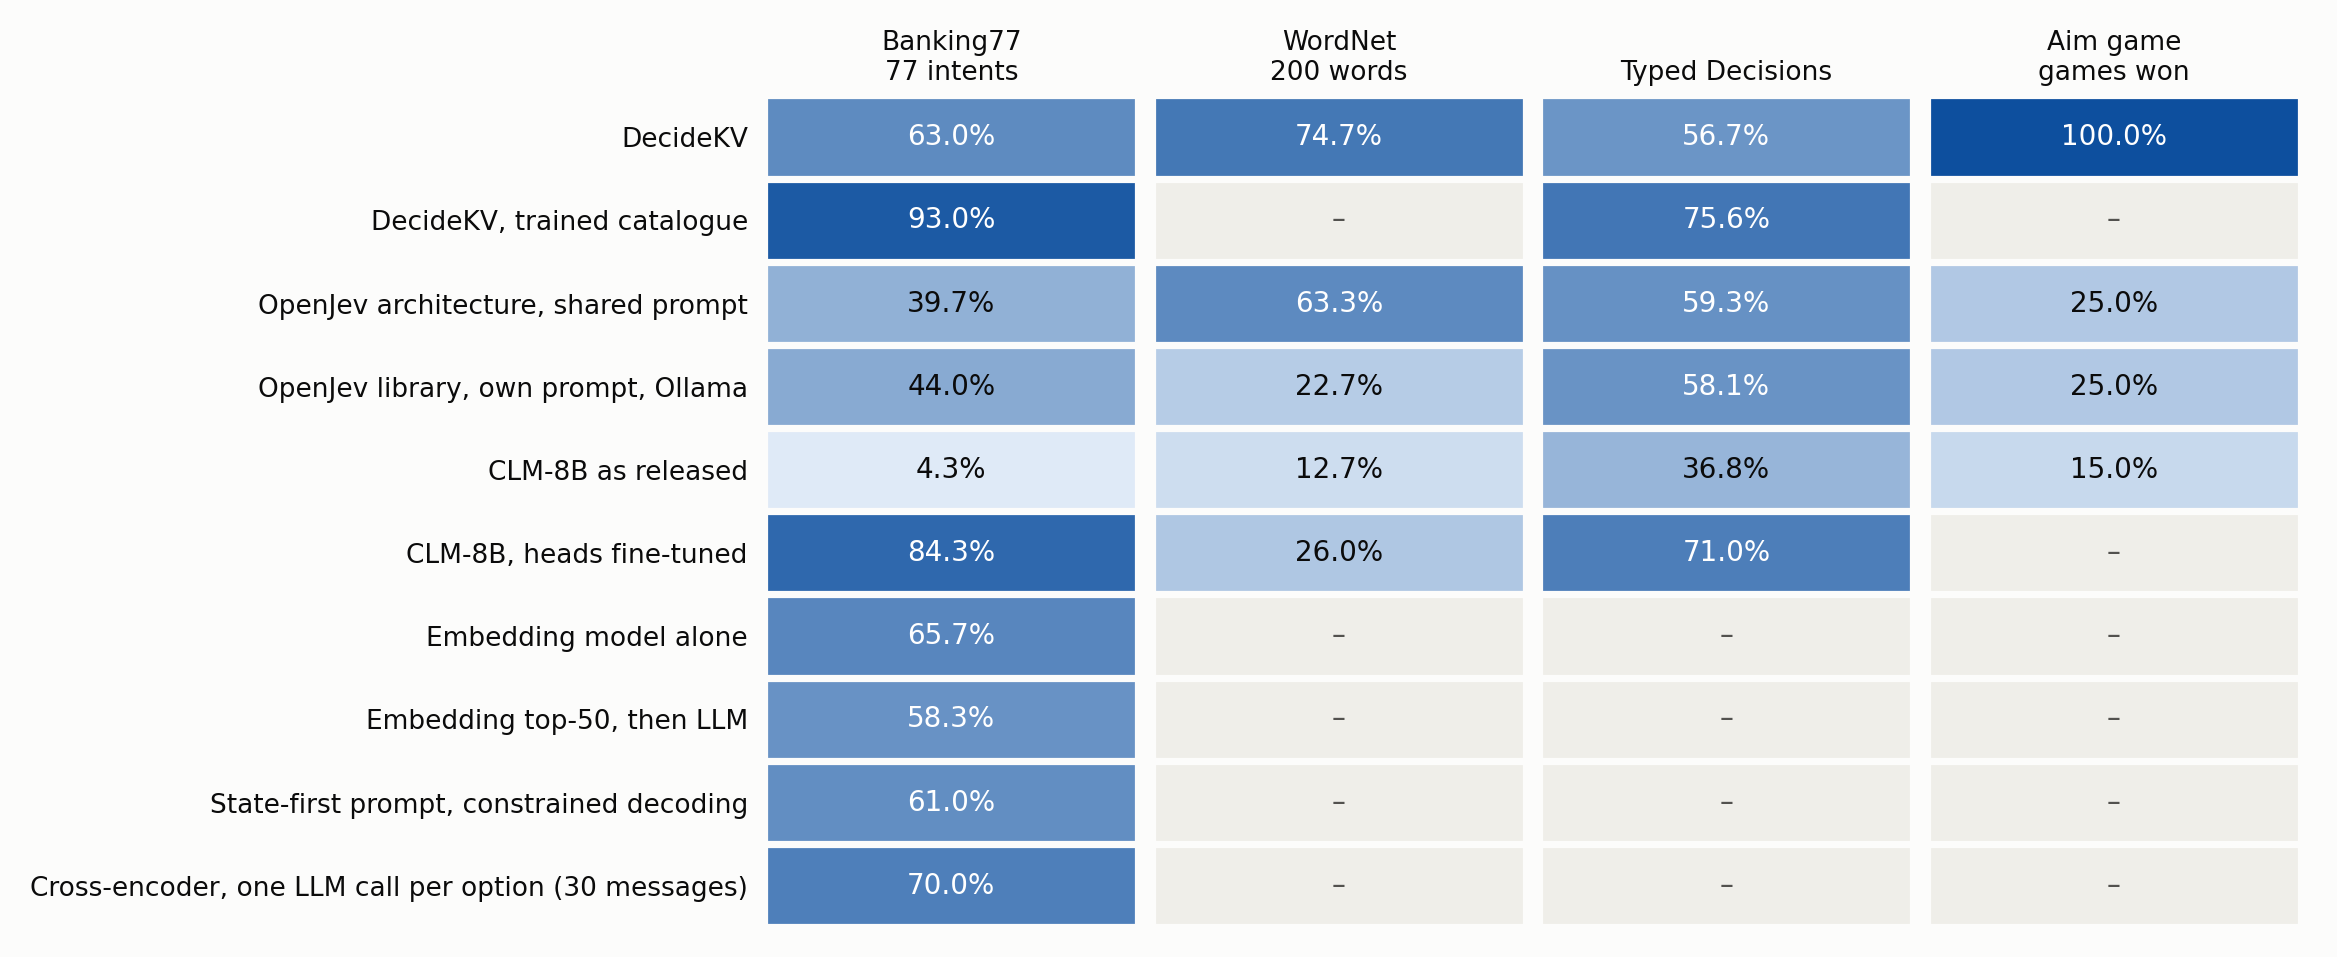
\includegraphics[width=0.95\linewidth]{fig_matrix.png}
\caption{Accuracy of every method on every task (Qwen3-8B).}\label{fig:matrix}
\end{figure}

\paragraph{Hybrid 27B model.} On Qwen3.8-27B (Table~\ref{tab:hybrid}) the resident prefix is the only reuse
available. \dkv{} is ahead of the OpenJev architecture on Banking77, WordNet-200 and Typed Decisions, and 1.6--5.7
times faster; on the aim game the OpenJev design did not finish in two hours because the whole grid is
recomputed at every shot, while \dkv{} won every game at 339\ms{} per shot. CLM-8B cannot run here: its heads belong
to Qwen3-8B.

\begin{table}[t]
\centering\small
\caption{Qwen3.8-27B (hybrid, IQ2\_S), context of 8{,}192 tokens for Typed Decisions and the aim game. Bold:
the best accuracy and the lowest time of each column.}\label{tab:hybrid}
\begin{tabular}{lllll}
\toprule
Method & Banking77 & WordNet-200 & Typed Decisions & Aim game (won) \\
\midrule
\dkv & \textbf{72.0\%} $\cdot$ \textbf{163\ms} & \textbf{84.7\%} $\cdot$ \textbf{106\ms} & \textbf{70.4\%} $\cdot$ \textbf{193\ms} & \textbf{100\%} $\cdot$ \textbf{339\ms} \\
OpenJev architecture & 45.7\% $\cdot$ 409\ms & 84.0\% $\cdot$ 600\ms & 69.1\% $\cdot$ 307\ms & $>$2\,h, stopped \\
\bottomrule
\end{tabular}
\end{table}

\subsection{Growing lists}
On the WordNet reverse dictionary with 150 definitions (Table~\ref{tab:scale}), \dkv{} keeps working where OpenJev
stops (255 options) and where the list no longer fits in memory; the catalogue takes over above 3{,}000 options and
keeps the right word among its 50 candidates in 86--90\% of the cases. Accuracy on an open vocabulary falls as the list
grows, for every method.

\begin{table}[t]
\centering\small
\caption{WordNet reverse dictionary, 150 definitions, Qwen3-8B.}\label{tab:scale}
\begin{tabular}{rllll}
\toprule
Options & \dkv & OpenJev arch. & CLM-8B & CLM-8B fine-tuned \\
\midrule
200 & 74.7\% $\cdot$ 37\ms & 63.3\% $\cdot$ 132\ms & 12.7\% $\cdot$ 21\ms & 26.0\% $\cdot$ 21\ms \\
1{,}000 & 58.7\% $\cdot$ 39\ms & not supported & 4.7\% $\cdot$ 21\ms & 16.7\% $\cdot$ 21\ms \\
3{,}000 & 60.7\% $\cdot$ 46\ms & not supported & 4.0\% $\cdot$ 21\ms & 10.7\% $\cdot$ 21\ms \\
10{,}000 & 52.7\% $\cdot$ 81\ms & not supported & 3.3\% $\cdot$ 21\ms & 8.7\% $\cdot$ 21\ms \\
30{,}000 & 48.0\% $\cdot$ 89\ms & not supported & -- & -- \\
\bottomrule
\end{tabular}
\end{table}

\subsection{Resident prefixes and the prefix tree}
On 100 Banking77 messages a resident list costs 64\ms{} per decision on Qwen3-8B against 155\ms{} when the prompt is
recomputed, and 157\ms{} against 538\ms{} on the 27B hybrid. Table~\ref{tab:order} shows the effect of the prompt order
on Typed Decisions: answering the five questions of a case in one call with the state first is more accurate and
faster than one question per call with the options first, on both models. Table~\ref{tab:turn} shows a turn of 15
questions: the prefix tree makes the state-first order faster even with a very short state, and 7.7 times faster with
a long state on Qwen3-8B (7.8 times on the 27B). Questions answered by option name are decoded token by token and stay
outside the batch.

\begin{table}[t]
\centering\small
\caption{Prompt order on Typed Decisions (2{,}000 decisions). Bold: the best accuracy and the lowest time of each column.}\label{tab:order}
\begin{tabular}{lll}
\toprule
& Qwen3-8B & Qwen3.8-27B \\
\midrule
Options first, one question per call & 51.0\% $\cdot$ 62\ms & 69.6\% $\cdot$ 249\ms \\
State first, five questions per call (prefix tree) & 56.7\% $\cdot$ \textbf{41\ms} & \textbf{70.4\%} $\cdot$ \textbf{193\ms} \\
OpenJev architecture & \textbf{59.3\%} $\cdot$ 67\ms & 69.1\% $\cdot$ 307\ms \\
\bottomrule
\end{tabular}
\end{table}

\begin{table}[t]
\centering\small
\caption{One turn of 15 questions (4 \texttt{Score}, 11 \texttt{Noul}) about one state; every turn has a new state.}\label{tab:turn}
\begin{tabular}{lrr}
\toprule
& Short state (99 chars) & Long state (3{,}177 chars) \\
\midrule
Qwen3-8B, options first & 337\ms & 2{,}615\ms \\
Qwen3-8B, prefix tree & \textbf{174\ms} & \textbf{338\ms} \\
Qwen3.8-27B, options first & 1{,}198\ms & 11{,}179\ms \\
Qwen3.8-27B, prefix tree & \textbf{763\ms} & \textbf{1{,}440\ms} \\
\bottomrule
\end{tabular}
\end{table}

\subsection{Trained catalogue}
On Banking77 the trained catalogue alone rises from 65.7\% to 93.0\% at the cost of one embedding (92\,s of training
on 10{,}003 examples, 17\,s of which optimisation). After training, sending its top-5 to the LLM \emph{lowers} the
accuracy (61.0\%): the untrained LLM re-chooses among good candidates and is worse than the catalogue. On Typed
Decisions (Table~\ref{tab:typed}) the catalogue trained on the official distributions reaches 75.6\% without any LLM
call, the most accurate method we measured on this task. Trained on the LLM's own answers, with no human label, it
reproduces its teacher: 50.4\% for the 8B teacher (which scored 51.1\% when labelling) and 66.6\% for the 27B
teacher (69.6\%), at 57\ms{} per decision instead of 188--249\ms.

\begin{table}[t]
\centering\small
\caption{Trained catalogue on Typed Decisions (catalogue alone, no LLM call unless stated). Bold: the best accuracy and the lowest time.}\label{tab:typed}
\begin{tabular}{lll}
\toprule
Catalogue & Labels & Accuracy $\cdot$ time \\
\midrule
Untrained & none & 44.5\% $\cdot$ 57\ms \\
Trained, hard labels & 6{,}000 human & 75.4\% $\cdot$ 57\ms \\
Trained, soft labels & 6{,}000 human & \textbf{75.6\%} $\cdot$ 57\ms \\
Trained on Qwen3-8B's answers & none & 50.4\% $\cdot$ 57\ms \\
Trained on Qwen3.8-27B's answers & none & 66.6\% $\cdot$ 57\ms \\
State embedded once, soft labels & 6{,}000 human & 67.2\% $\cdot$ \textbf{9\ms} \\
\midrule
\dkv{} with Qwen3-8B (LLM) & none & 56.7\% $\cdot$ 41\ms \\
\dkv{} with Qwen3.8-27B (LLM) & none & 70.4\% $\cdot$ 193\ms \\
CLM-8B, heads fine-tuned & 6{,}000 human & 71.0\% $\cdot$ 79\ms \\
\bottomrule
\end{tabular}
\end{table}

\paragraph{Fallback.} With a head trained on the examples of half of the Banking77 intents, intents without examples
fall to 21.1\%. With the fallback they rise to 61.2\% (64\% of these decisions go to the LLM), while intents with
examples go from 95.4\% to 85.0\%; over all 300 messages, 59.0\% becomes 73.3\% (untrained catalogue: 65.7\%).

\paragraph{Cascade.} On Typed Decisions with the 27B model and a head trained on the 27B's own answers, a threshold
of 0.5 gives 71.3\% in 251\ms{} against 70.2\% in 260\ms{} for the LLM alone; at 0.3, 68.9\% in 191\ms{} with
half of the questions answered by the head alone. With a head trained on human labels, which is more accurate than the
LLM, every question sent to the LLM lowers the accuracy: a cascade pays when the LLM is the better judge. (The 27B and
the encoder do not fit together in 12\,GB, so the cascade was run in two phases with the same arithmetic.)

\subsection{Question before the state}
With the options first, the question can go before the state (one constant prefix: instructions, options, question)
or after it. Each message was answered in both orders with the same model; Table~\ref{tab:qfirst} counts, for the
paired McNemar test, the messages answered right in only one of the two. The question before the state is never less
accurate, is significantly more accurate on CLINC150~\citep{clinc}, and saves about eleven tokens per decision, so it
is the default when a list is asked its own question; all the results of Tables~\ref{tab:comparison}--\ref{tab:scale}
with one question per list use it.

\begin{table}[t]
\centering\small
\caption{Question after or before the state (Qwen3-8B, options first). Last columns: messages answered right only with
the question after / only with it before, and the McNemar $p$-value.}\label{tab:qfirst}
\begin{tabular}{lllcc}
\toprule
& After the state & Before the state & Only after / only before & $p$ \\
\midrule
Banking77 (3{,}080 messages) & 65.1\% $\cdot$ 66\ms & 65.5\% $\cdot$ \textbf{65\ms} & 72 / 85 & 0.34 \\
CLINC150 (4{,}500 messages) & 80.0\% $\cdot$ 55\ms & \textbf{81.4\%} $\cdot$ \textbf{54\ms} & 107 / 170 & 0.0002 \\
Typed Decisions (2{,}000) & 51.0\% $\cdot$ 66\ms & 51.1\% $\cdot$ \textbf{62\ms} & 133 / 136 & 0.90 \\
\bottomrule
\end{tabular}
\end{table}

\subsection{Semantic cache and the two modes}
A semantic cache reuses the LLM's answer for a state whose embedding has a cosine of at least a threshold with a state
already answered. Table~\ref{tab:semcache} runs it on streams of messages. On short natural-language messages
(Banking77, CLINC150) a threshold of 0.95 keeps the LLM's accuracy with 37--47\% of the answers reused; on structured
states (Typed Decisions) it loses accuracy even at 0.98, because states with almost the same text can need different
answers. The catalogue trained on the LLM's answers is 4--9 times faster than the LLM on short messages, from 4.5
points less accurate to slightly more. This gives two modes: for \emph{structured states}, the LLM with the prefix tree
and no cache; for \emph{short natural-language messages}, a trained catalogue for speed, or the LLM with the cache
(\texttt{cache=0.95}) to keep exactly its answers.

\begin{table}[t]
\centering\small
\caption{Semantic cache on streams of messages (Qwen3-8B): accuracy $\cdot$ mean time per decision, with the share of
answers reused. Last column: the catalogue trained on the LLM's answers (for Typed Decisions, the 8B-taught catalogue of
Table~\ref{tab:typed}).}\label{tab:semcache}
\resizebox{\linewidth}{!}{\begin{tabular}{llllll}
\toprule
& LLM alone & Cache 0.98 & Cache 0.95 & Cache 0.90 & Trained catalogue \\
\midrule
Banking77 (3{,}300) & 62.5\% $\cdot$ 67\ms & 62.7\% (10\%) & 62.5\% $\cdot$ 57\ms{} (37\%) & 62.6\% $\cdot$ 36\ms{} (69\%) & 58.0\% $\cdot$ 15\ms \\
CLINC150 (4{,}500) & 79.8\% $\cdot$ 53\ms & 79.7\% (17\%) & 80.0\% $\cdot$ 34\ms{} (47\%) & 77.9\% $\cdot$ 20\ms{} (74\%) & 80.3\% $\cdot$ 6\ms \\
Typed Decisions (8{,}000) & 57.9\% $\cdot$ 42\ms & 56.1\% (16\%) & 53.1\% $\cdot$ 21\ms{} (54\%) & 50.2\% $\cdot$ 9\ms{} (81\%) & 50.4\% $\cdot$ 57\ms \\
\bottomrule
\end{tabular}}
\end{table}

\subsection{Negative results}
\begin{itemize}
\item \textbf{Embedding the state once} per call and putting the question in the cached option texts is 6.4 times
faster (9\ms{} per decision) but loses 6--8 points of accuracy (67.2\% instead of 75.6\% with human labels); it is
an option, not the default.
\item \textbf{Linear heads on the LLM's last hidden state} of the state, one per question, reach 68.9\% in 14\ms{}
on Qwen3-8B and 66.7\% in 52\ms{} on the 27B: below fine-tuned CLM-8B (whose method this essentially is) and below
the trained catalogue, so we did not include them.
\item \textbf{An identity regulariser} on the low-rank correction improved the accuracy on intents without examples
only from 15\% to 28\% at best.
\item \textbf{The confidence margin} between the first and the second option could not flag the head's errors on
intents without examples: those errors are made with high confidence.
\end{itemize}

\section{Limitations}
Probabilities computed by llama.cpp depend on how the prompt is split into batches (the kernels are not
batch-invariant): on Qwen3-8B the same prompt evaluated whole, in two pieces or token by token gave the most probable
answer of an uncertain \texttt{Noul} question between 0.76 and 0.93, also on CPU and with flash attention off
(smaller, but not zero). Resident prefixes and the prefix tree only change where the prompt is split; they are exact
with respect to the same split, and confident answers do not move. All results come from one GPU and one model family
(Qwen); the OpenJev library and CLM rows were not re-measured under the shared prompt; the trained catalogue was
measured on two datasets; on hybrid models the eight-sequence limit of llama.cpp bounds the parallelism of the tree;
and \texttt{full=True} costs about 2.3\,s on the 27B hybrid.

\section{Related work}\label{sec:related}
\textbf{Candidates in the context and cache reuse.} Placing the candidates first so that they are encoded once is the
corpus-in-context setting of LOFT~\citep{loft}; reusing a precomputed KV cache across queries is cache-augmented
generation~\citep{cag}. Serving systems share prefixes across requests with paged or radix-tree caches
(vLLM~\citep{vllm}, SGLang~\citep{sglang}, ChunkAttention~\citep{chunkattention}) and speed up attention over shared
prefixes (Hydragen~\citep{hydragen}); \dkv{} applies the same principle inside one process to decision workloads, with
explicit resident sequences that also work on hybrid recurrent models.
\textbf{Constrained decoding.} Decoding through a trie of candidate names follows GENRE~\citep{genre}; grammar-based
decoding is common in structured generation~\citep{outlines}.
\textbf{Typed decisions.} Jev-style systems and OpenJev~\citep{openjev} define the \texttt{Choice}/\texttt{Score}/\texttt{Noul}
interface that \dkv{} implements. Contrastive Language Models~\citep{clm} train heads on top of an LLM; our trained
catalogue instead corrects a frozen embedding space and leaves the LLM untouched.
\textbf{Concurrent work.} SharedKV-BT~\citep{sharedkvbt} encodes the context of a behaviour-tree node once and scores the
candidates of all its fields in one batch (Hugging Face Transformers, 3--4B models), reporting 2.4--4.2$\times$ speedups
over constrained decoding. LLM-as-Jev~\citep{llmasjev} answers \texttt{Choice}/\texttt{Score}/\texttt{Noul} by prefill
alone, sharing prefixes within a request, and studies fine-tuning of the LLM. Both share the idea of scoring several
questions over a context encoded once, which our prefix tree also uses; neither keeps option lists resident across
states, switches to an embedding catalogue for large lists, trains a catalogue (from human labels or from the LLM),
or targets hybrid recurrent models. We found these works after our implementation was written.
\textbf{Contrastive training.} The catalogue objective is InfoNCE~\citep{infonce,clip} with soft targets, and its
low-rank, identity-initialised correction follows LoRA~\citep{lora}.

\section{Future work}
In our aim game the target does not move, so the state is the current grid and the options are fixed. With moving
targets---interception in robotics, pedestrians in autonomous driving, demand in logistics, load in energy networks,
leading shots in games---the decision should be taken on where the target \emph{will be}, not where it is. A natural
sequel is to put a time-series forecaster in front of \dkv: the forecaster produces the predicted state, and the
decision is taken on it with the same resident options and prefix tree; temporal patterns may also help to group
similar states. Predict-then-act designs exist in robotics, where a small world model forecasts future visual tokens
for a frozen vision-language-action model and enables catching moving objects~\citep{ahead}, and LLM agents are
increasingly combined with time-series models~\citep{tsagents}; we are not aware of work that pairs a forecaster with
typed, cache-resident LLM decisions under a latency budget.

\section{Conclusion}
\dkv{} is a free tool for a frequent task: fast, constrained, typed decisions with a local LLM. It is ready to use
with any GGUF model, much faster than the OpenJev architecture and at least as accurate in six of seven
comparisons, it scales to tens of thousands of options, it needs no training, and it can be trained
like CLM---from human labels or from the LLM itself---to answer in milliseconds without calling the LLM. Its weaknesses
are stated above and in the repository. Treating typed decisions as a KV-cache problem---keep what is shared, compute
what changes, branch where questions diverge---is the idea behind it. The library, the benchmarks and every result file
are at \url{https://github.com/HGarrone/decidekv}.

\paragraph{Use of AI assistants.} The code of the library was written by a local code model (qwen3-coder-30B) under
the author's direction; an AI assistant (Claude) helped with the design, the verification of the code and of the
measurements, and the writing of this paper. The author chose the experiments, checked the results and takes
responsibility for the content.

\bibliographystyle{plainnat}
\bibliography{refs}

\end{document}
